%
% file: localoperator.tex
% author: Victor Brena
% description: Briefly describes properties of the local operator.
%

\chapter{Function Failure Identification and Propagation}
\label{app:app04}

\initial{S}everal initiating events are considered, and the propagation of the failures is computed using FFIP methodology. The loss of the function \textit{Signal - Sense - Measure} linked to the \textit{Energy - Radioactive} flow is propagated on figure~\ref{fig:ffip1}. This is equivalent to the loss of neutron detectors in a RBD. Next, the loss of the function {Channel - Guide - Rotate}, which connect the flow \textit{Material - Gas} with \textit{Energy - Mechanical} is propagated on figure~\ref{fig:ffip2}. This is equivalent to the loss of the turbines in a RBD. Furthermore, the loss of the function \textit{Convert - Convert} converting vapor flow to liquid flow is propagated on figure~\ref{fig:ffip3}. THis is equivalent to the loss of the condensers in a RBD.

Two critical functions are defined. These functions are the one that are critical to the system reliability (electricity generation) and the system risks (preventing a core meltdown).

\begin{figure}[t]
\centering
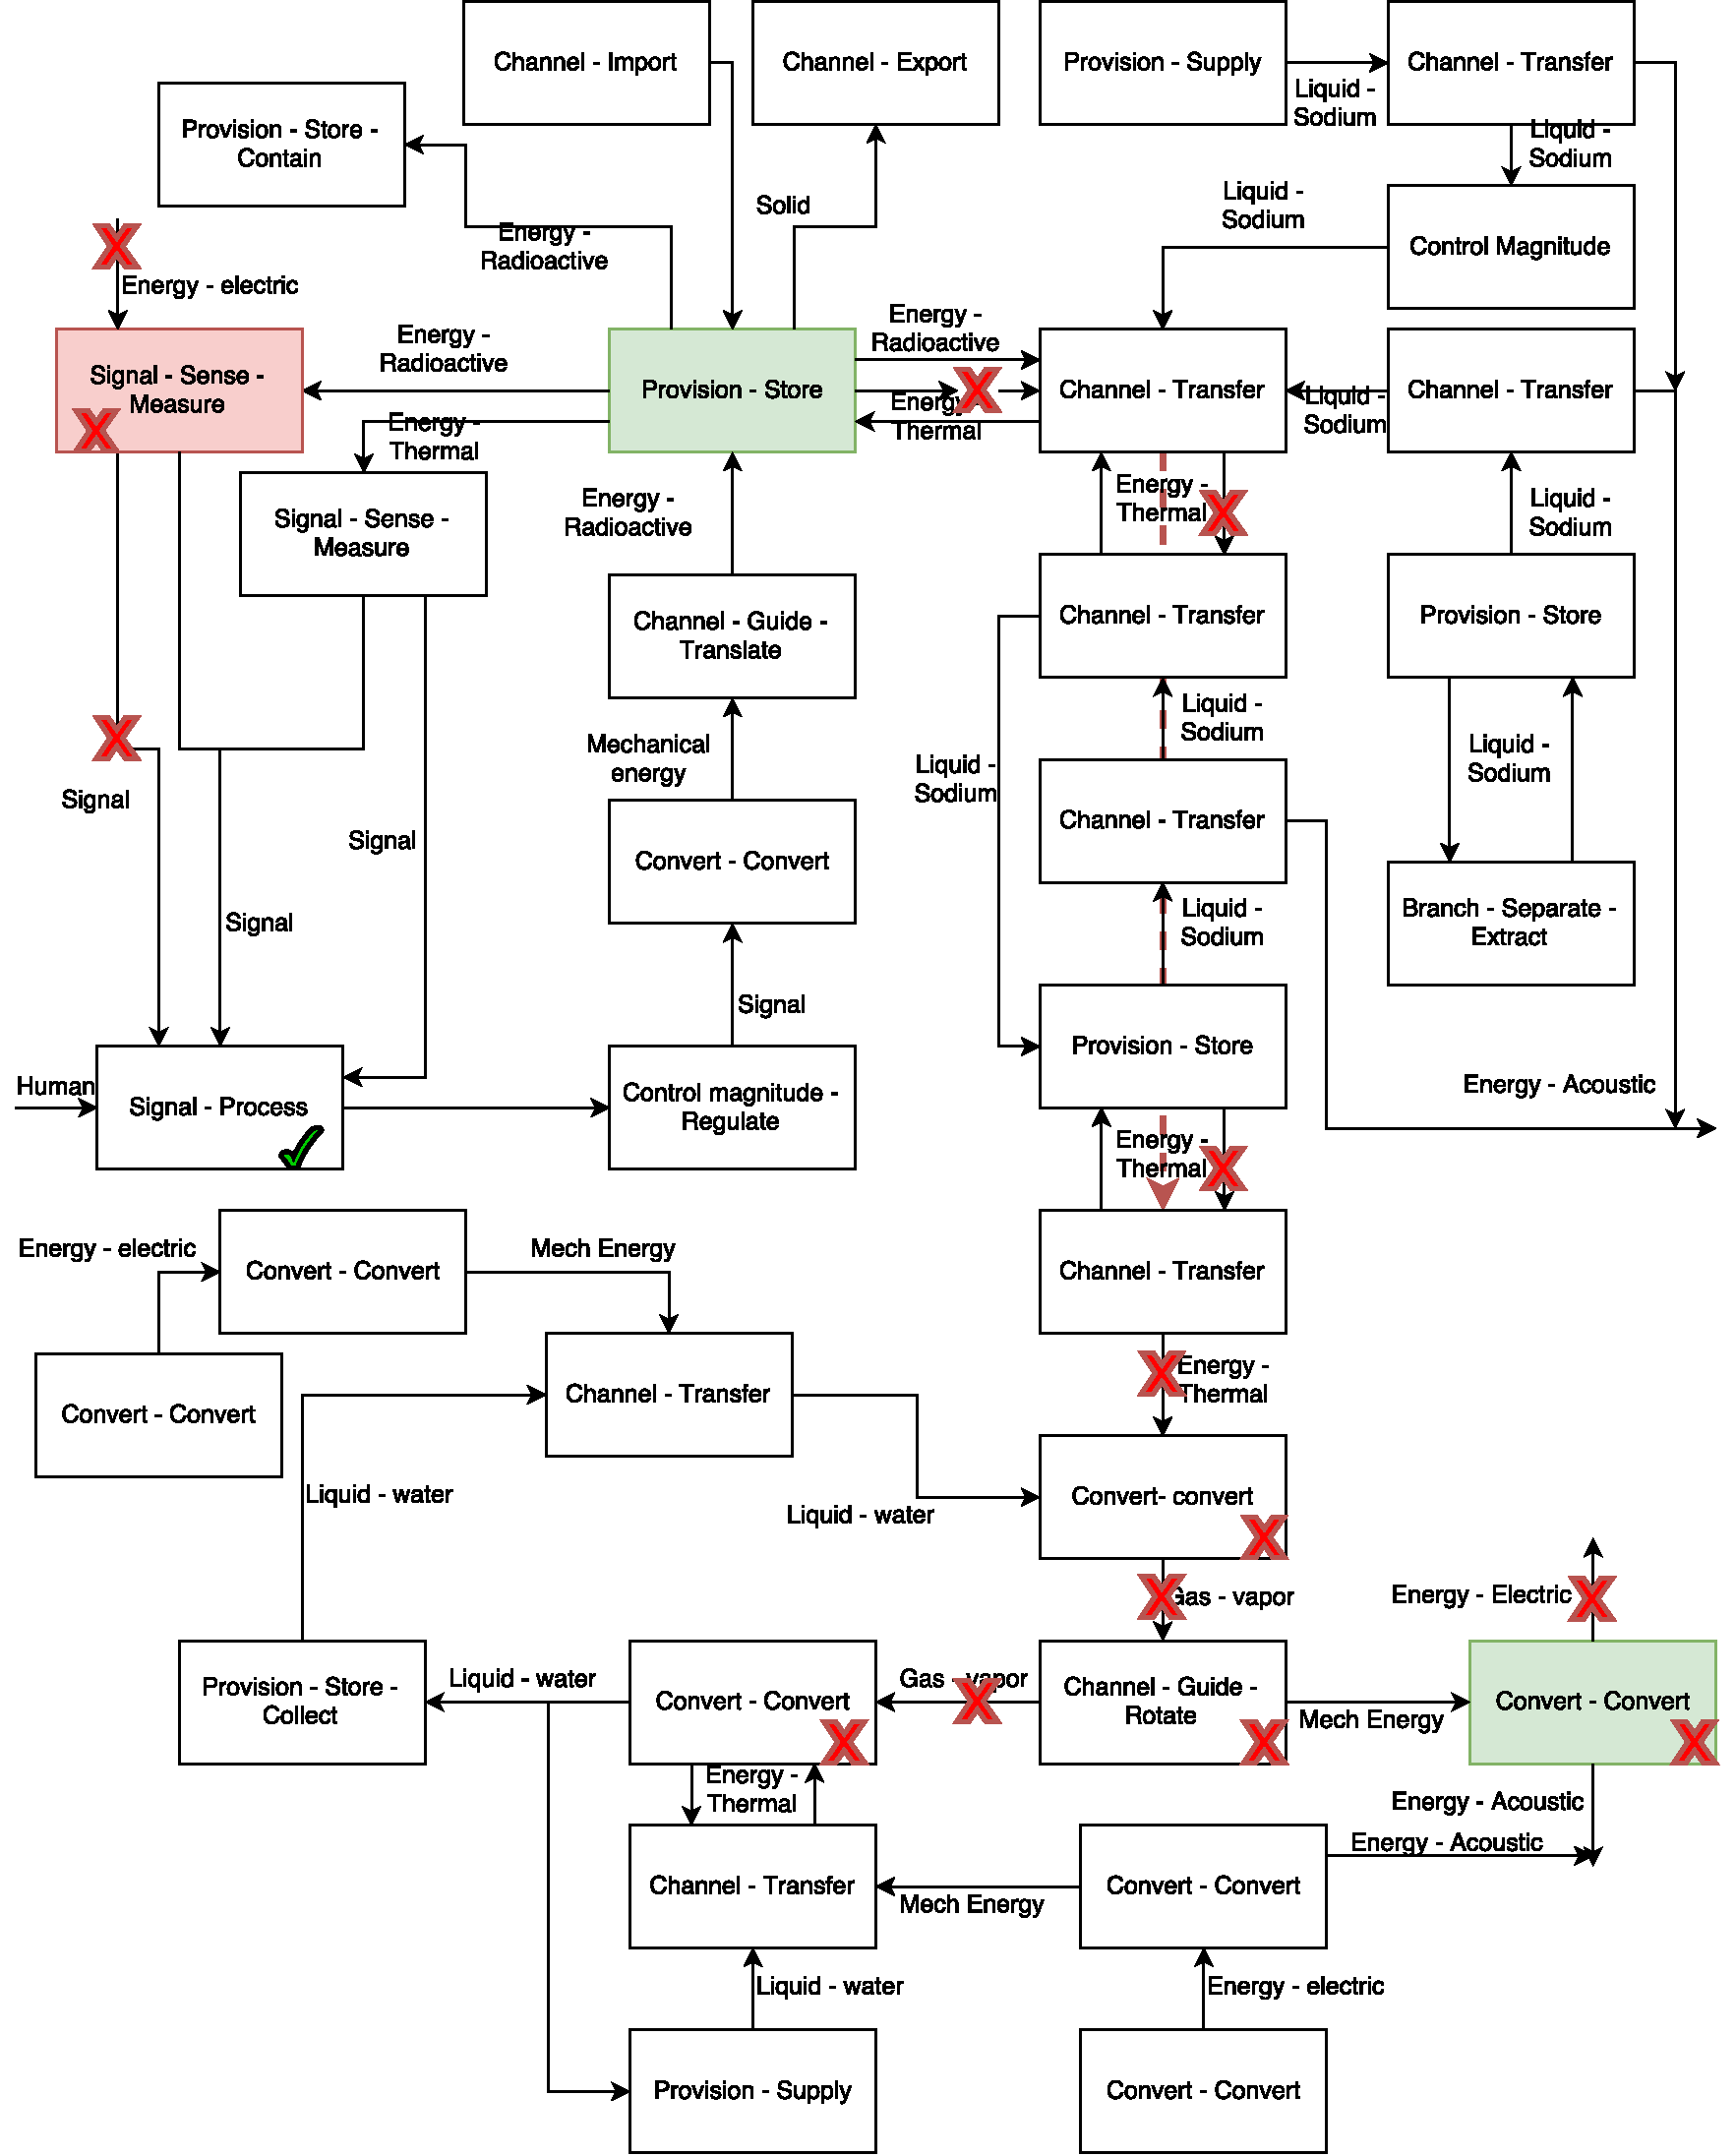
\includegraphics[scale=.55]{fig0d/FFIP_1}
\caption{FFIP - Initiating event: Loss of signal for the neutron detectors.}
\label{fig:ffip1}
\end{figure}

\begin{figure}[t]
\centering
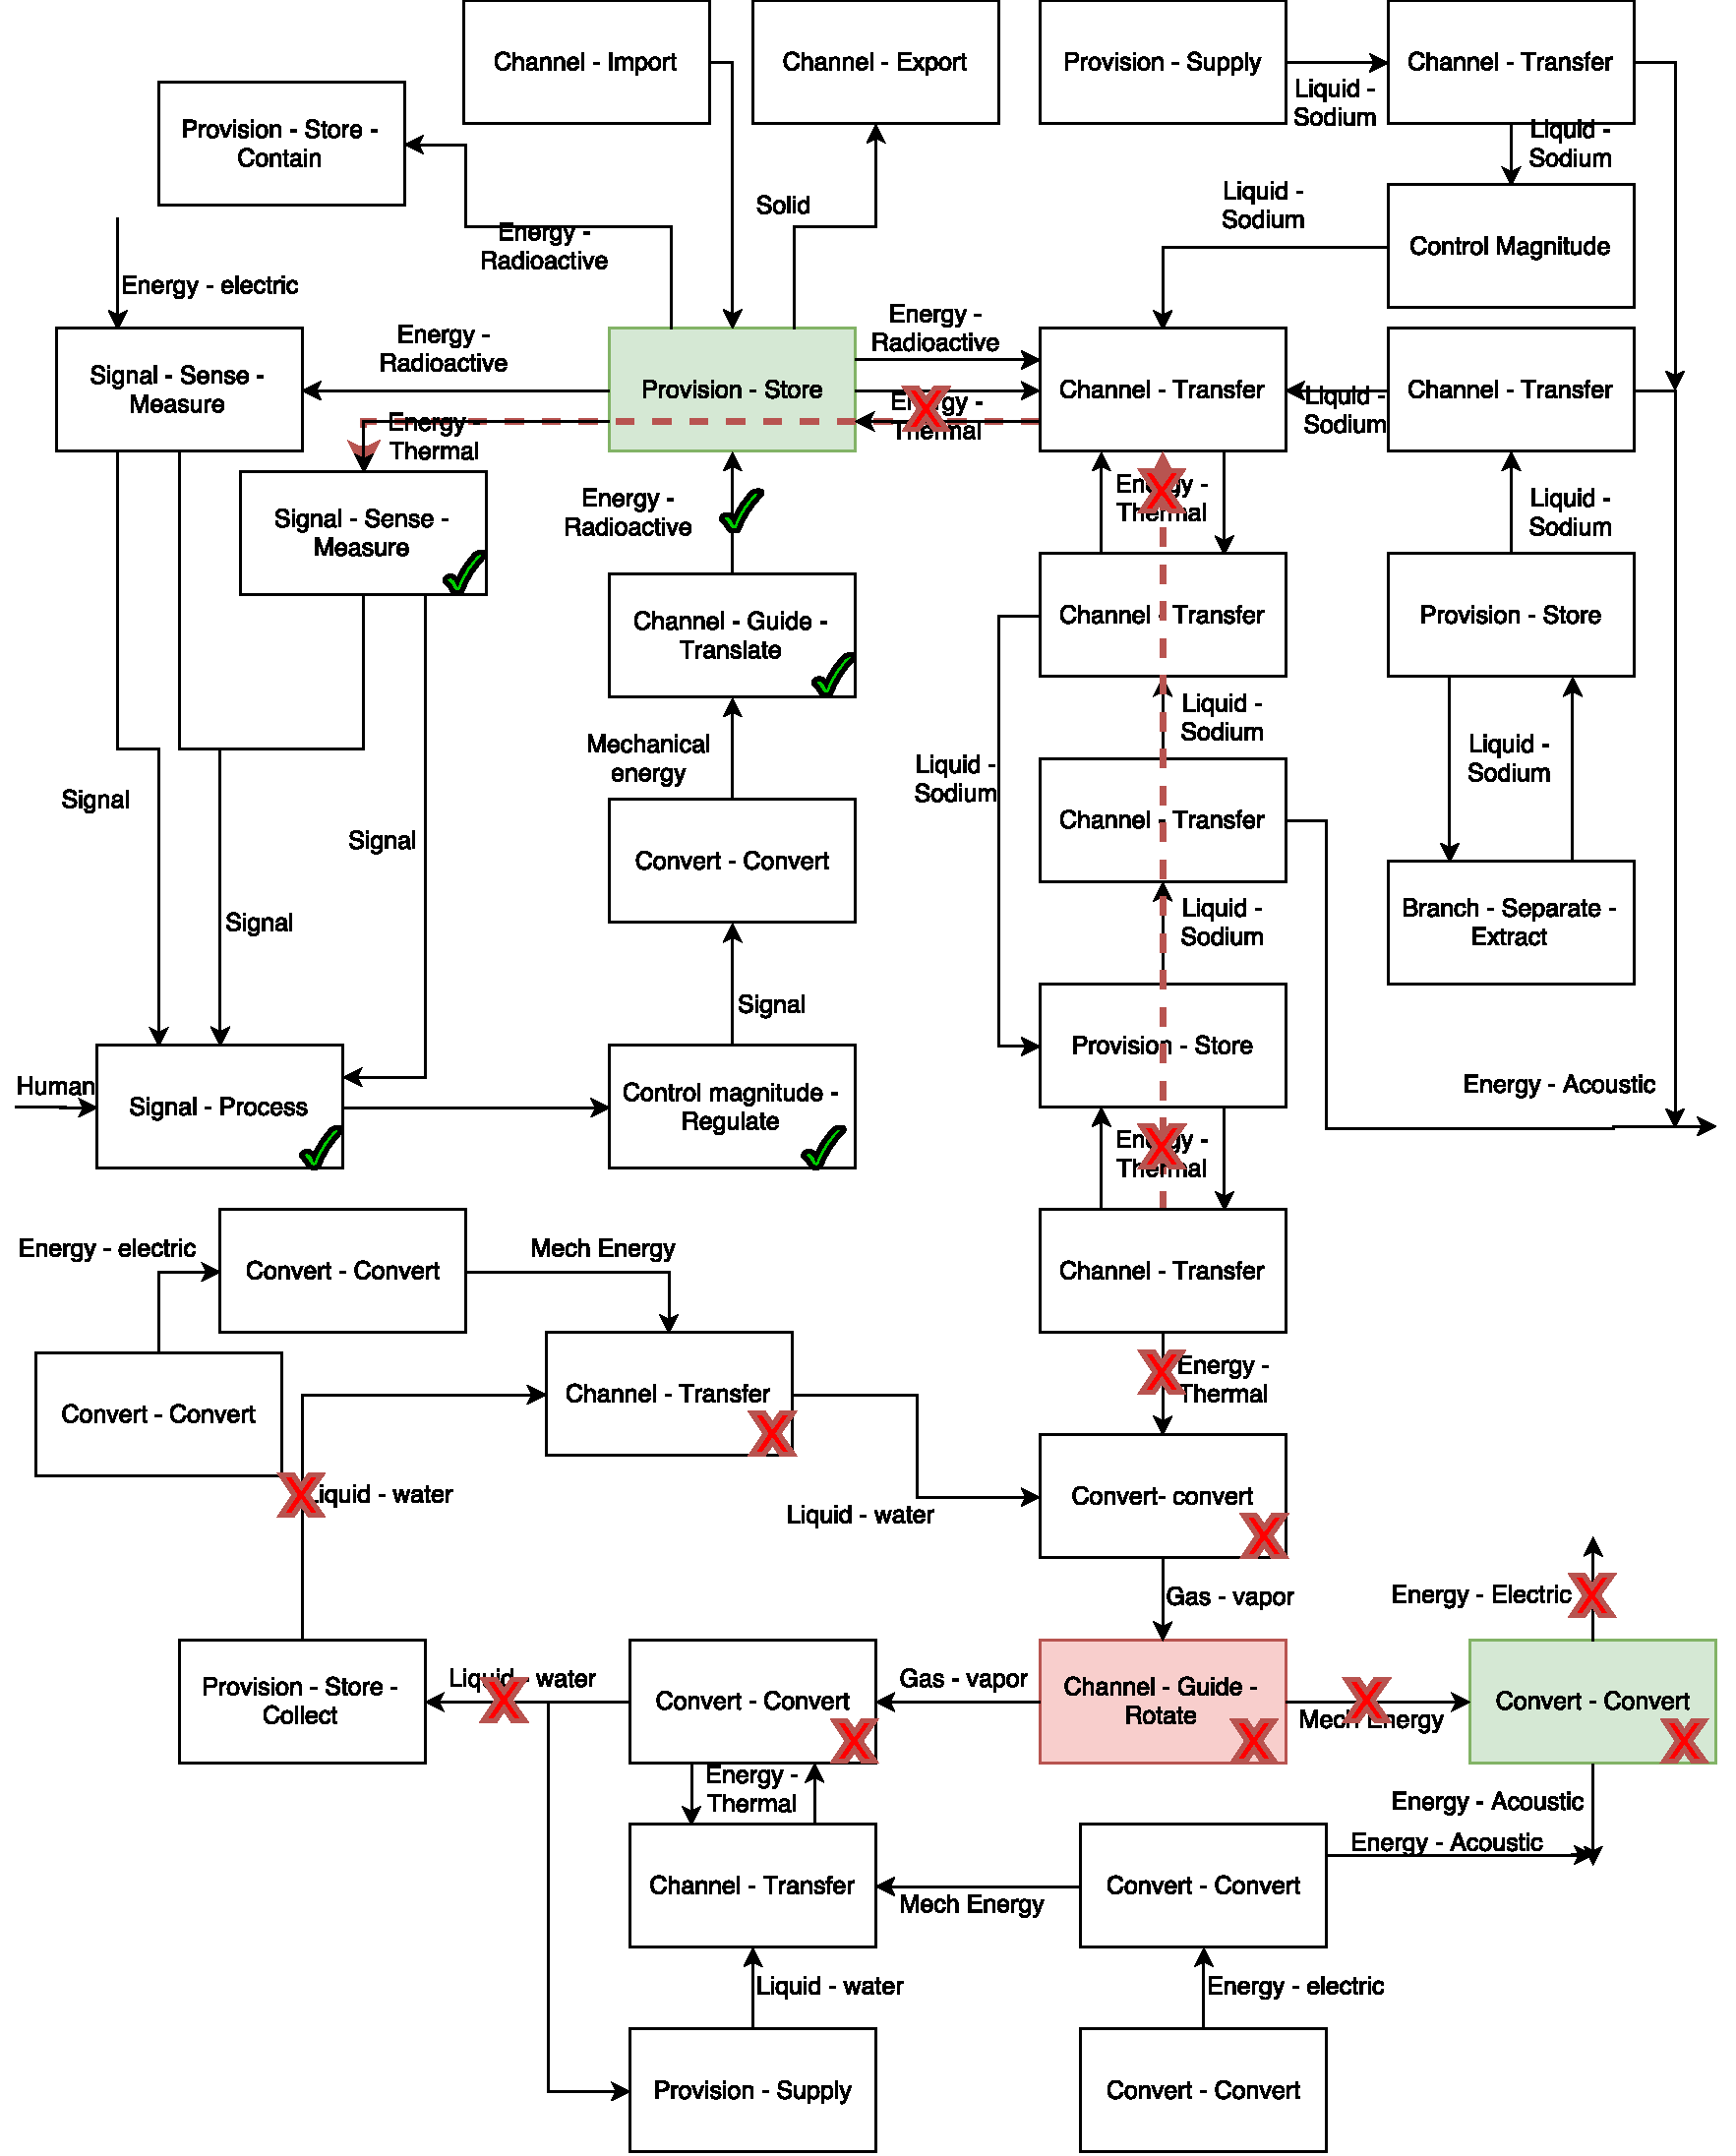
\includegraphics[scale=.55]{fig0d/FFIP_2}
\caption{FFIP - Initiating event: Loss of turbines.}
\label{fig:ffip2}
\end{figure}

\begin{figure}[t]
\centering
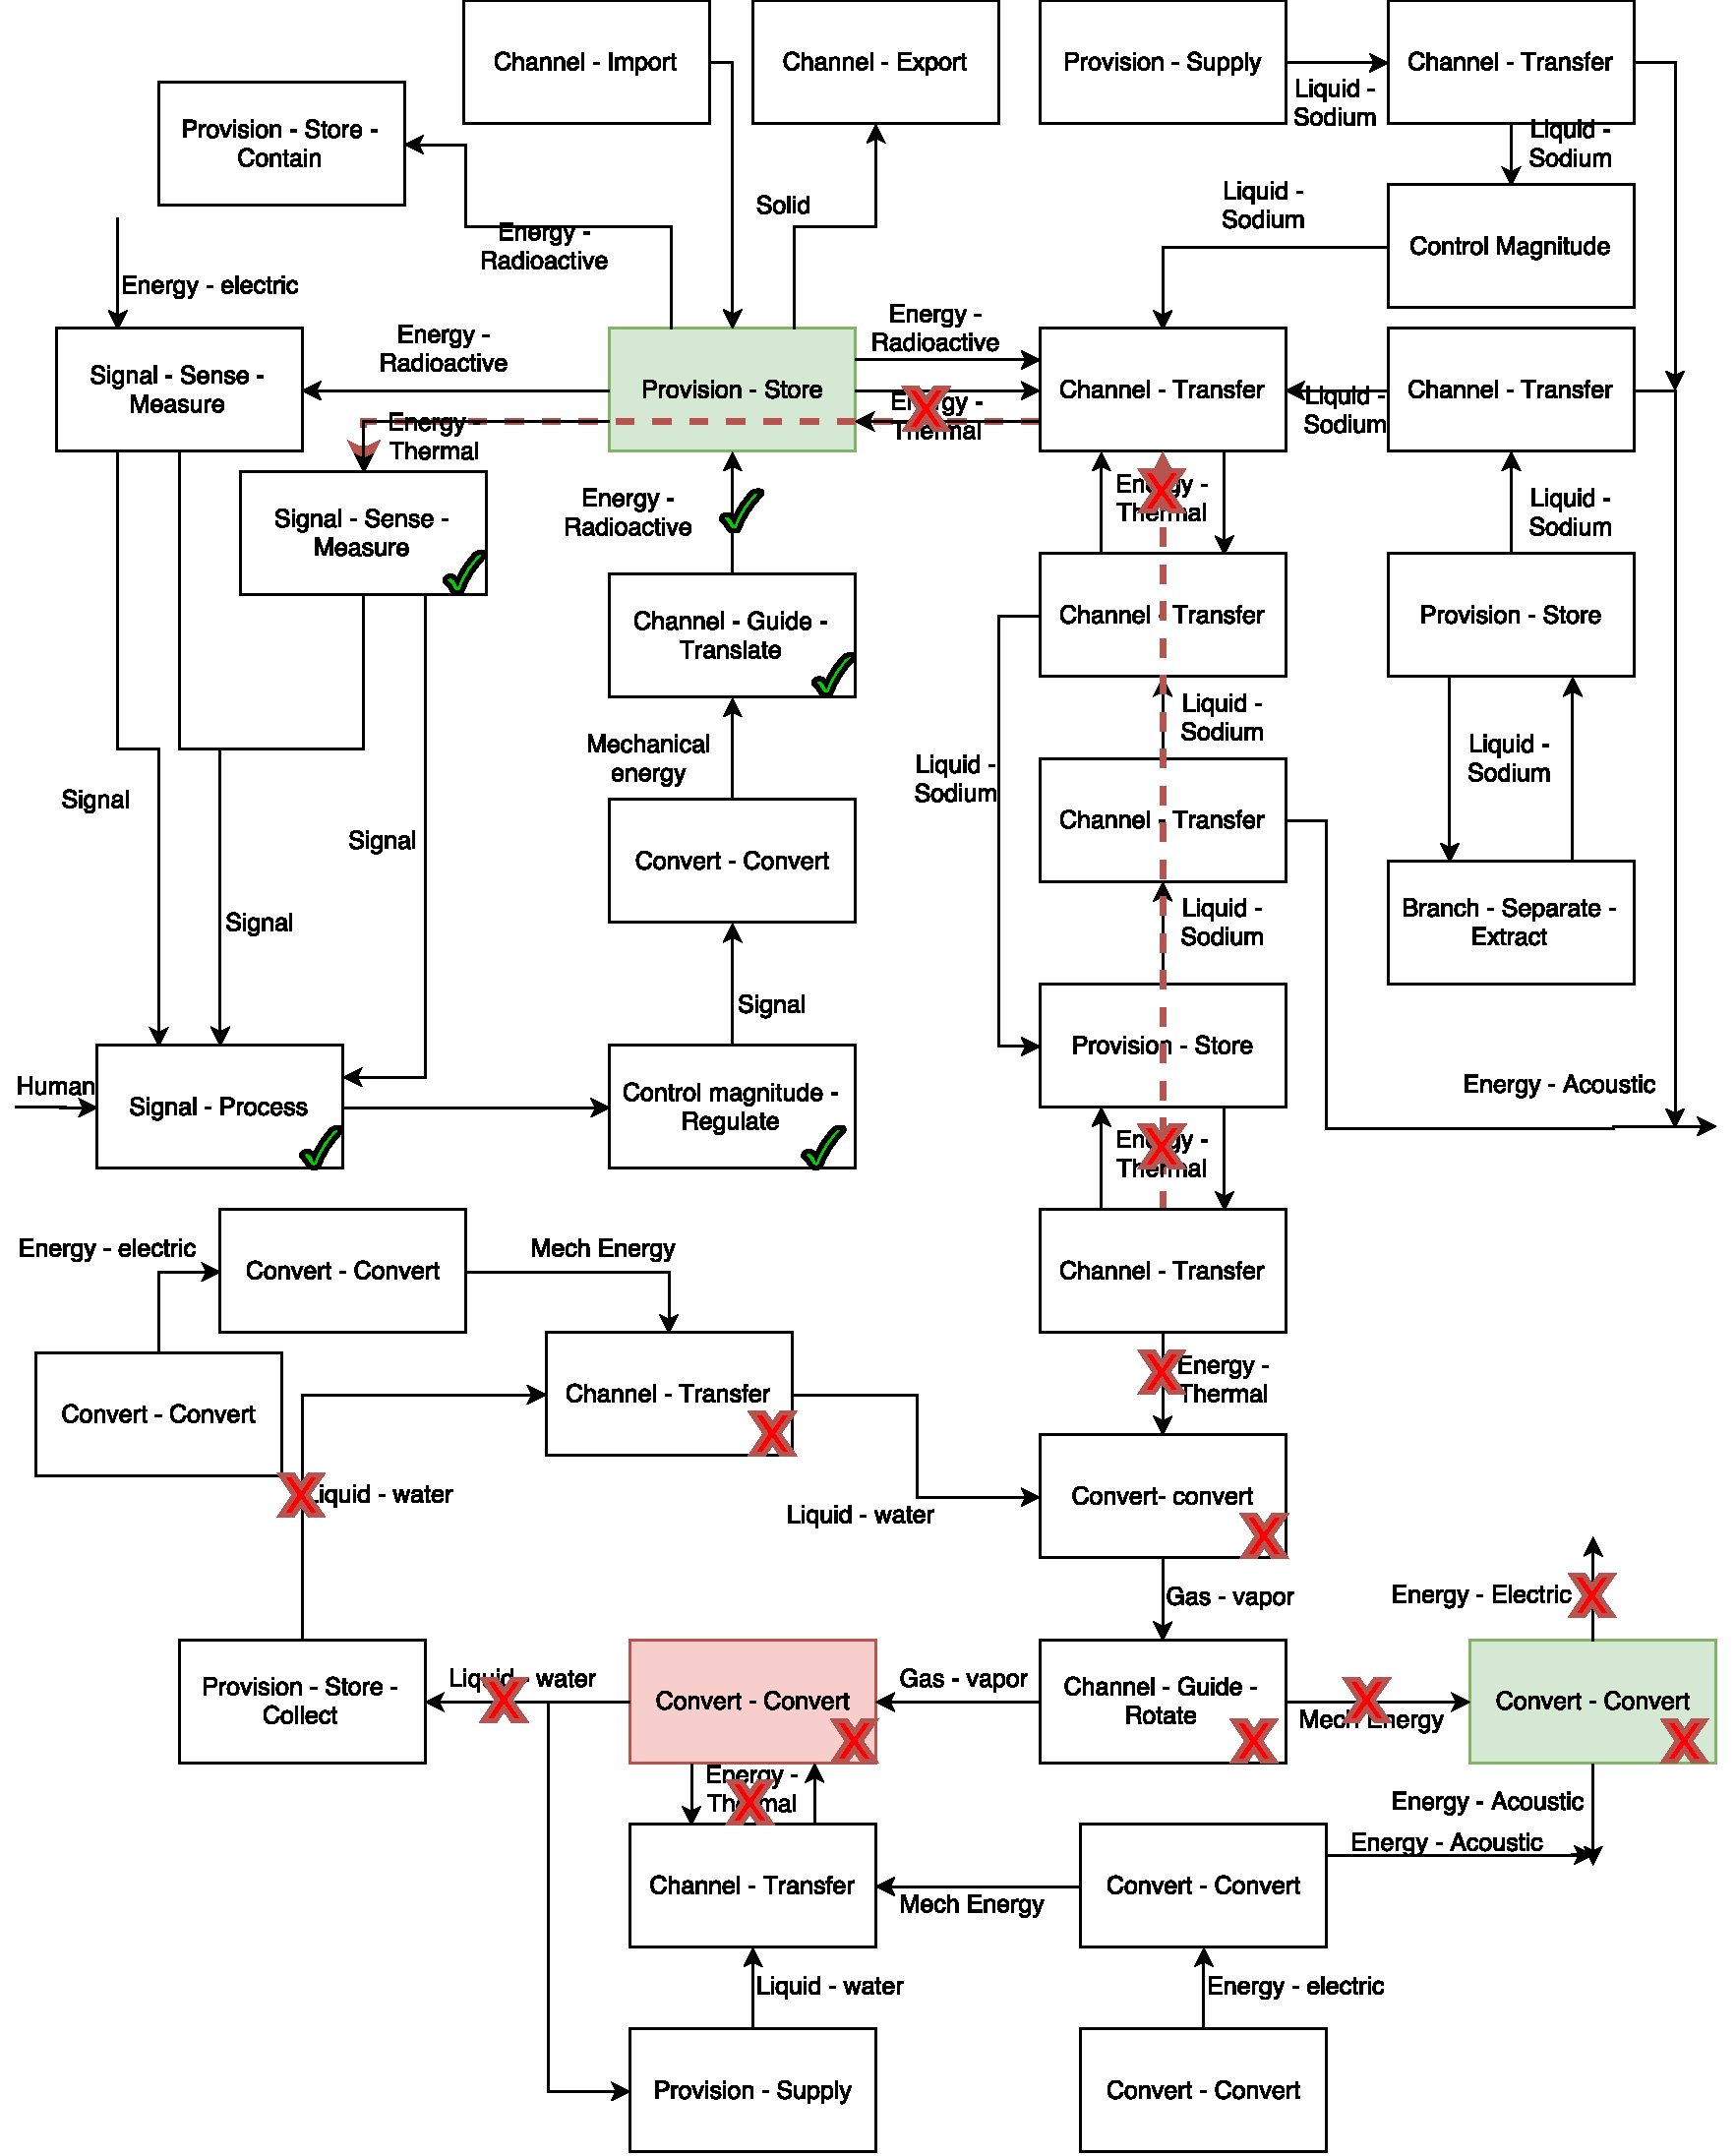
\includegraphics[scale=.55]{fig0d/FFIP_3}
\caption{FFIP - Initiating event: Loss of condensers.}
\label{fig:ffip3}
\end{figure}



\
